\documentclass{article}
\usepackage[utf8]{inputenc}
\usepackage[T1]{fontenc}

\title{Rapport Apprentissage Automatique}
\author{Gabin Marc Mberi-Kongo, Quentin Vigne, Vincent Deschaud}
\author{Thomas Cambon, Florent Jakubowski }
\author{
  Gabin Marc Mberi-Kongo\\
  \texttt{gabin.mberi-kongo@univ-lyon2.fr}
  \and
  Quentin Vigné\\
  \texttt{quentin.vigne@univ-lyon2.fr}
  \and
  Vincent Dechaud\\
  \texttt{vincent.dechaud@univ-lyon2.fr}
  \and
  Thomas Cambon\\
  \texttt{t.cambon@univ-lyon2.fr}
  \and
  Florent Jakubowski\\
  \texttt{florent.jakubowski@univ-lyon2.fr}
}
\date{February 2021}

\usepackage{natbib}
\usepackage{graphicx}

\begin{document}

\maketitle

\tableofcontents

\section{Introduction}

Dans le cadre du module Apprentissage supervisé dispensé par Monsieur Ah-pine, nous avons eu le choix d'implémenter un algorithme d'apprentissage supervisé parmi plusieurs et de tester ses performances par rapport à d'autres méthodes d'apprentissage supervisé. 

\section{Sujet}
Parmi les différents sujets proposés nous avons fait le choix de travailler sur le sujet "Adaboost" qui nécéssite d'étudier de façon approfondie deux algorithmes pour la catégorisation de données. Ces deux algorithmes porteront sur la catégorisation binaire et sur la catégorisation multiclasse. Afin de traiter ce sujet, une première étape de lecture et d'analyse de notre sujet et nécéssaire, notamment par la lecture des articles fondateurs de l'adaboost et de la prise de connaissance des notions de boosting.  
\section{Problématiques scientifiques}
La problématique scientifique pour ce projet est de vérifier l'intérêt des méthodes dites d'ensembles pour la classification binaire et multiclasses, plus spécifiquement l'algorithme Adaboost. L'enjeux sera d'observer la différence de performance entre des méthodes d'apprentissage supervisé ne se basant pas sur une prédiction par comité et des méthodes qui au contraire utilisent le vote par comité pour faire leur prédiction.
Nous sommes appuyés sur l'implémentation de l'algorithme adaboost et de sa variante l'algorithme Adaboost M1 telle que décrite dans l'article de Freund et Schapire \citep{FreundSchapire1996} en 1996 pour reimplémenter nos algorithmes.

\section{Fondements, principes et état de l'art}
Le fondement de l'Adaboost part du principe d'algorithmes de "Boosting" introduit par Yoav Freund et Robert Schapire en juillet 1996 \citep{FreundSchapire1996} dans l'article "Experiments with a new boosting algorithm". Le but de ce nouvel algorithme de boosting est de réduire significativement l'erreur générée par les classifieurs faibles qui donnent un score à peine meilleur qu'un classifieur aléatoire. Ces classifieurs sont dénommés "classifieurs faibles" ou bien "Weak Learner" dans l'article original. Ce fût la première méthode fonctionnelle permettant de mettre en oeuvre le principe de boosting.

Souvent le bagging et le boosting sont confondus puisque ces deux méthodes sont toutes les deux des méthodes ensemblistes. Le boosting que nous étudions ici va attribuer un poids plus fort aux classifieurs ayant prédit correctement que ceux dont la prédiction est incorrecte. Adaboost s'appuie sur ce principe en donnant plus d'importance aux valeurs compliquées à prédire. On booste les classifieurs qui réusissent lorsque d'autres échouent.


\section{Implémentation}
Le but de cette partie est d'explicité d'une part les détails techniques et l'organisation du code (5.1, 5.2, 5.4) et d'autre part notre organisation en tant qu'équipe et la manière dont nous avons réalisé ce code (5.3 Workflow)
le langage utilisé, le workflow, les différentes fonctions et leur spécification (comment avez-vous réalise, organisé votre code et avec quels outils ?)
\subsection{Langage et librairies utilisés}
Nous avons utilisé le langage python pour développer notre code. Ce choix a été motivé par la simplicité d'implémentation et de compréhension du code, de plus l'accès à de nombreuse librairies comme panda ou scikit-learn était très intéressant dans notre cas. 

Ci-suit la liste des librairies python utilisées dans ce projet : 
\begin{itemize}
  \item Numpy : Numpy est une bibliothèque que nous utilisons pour le calcul matricielle et sur des tableaux de plusieurs dimensions.
  \item Pandas : Pandas est une bibliothèque permettant de manipuler des données également en python. Nous nous en servons pour charger des données depuis un csv dans des dataframe pandas et pouvoir ensuite effectuer des opérations dessus.
  \item Scikit-learn : Scikit-learn est une bibliothèque destiné à l'apprentissage automatique. Elle fournit de nombreuses classes d'algorithmes d'apprentissage supervisé très simple à manipuler, des fonctions pour séparer son jeu de données en deux jeu de données d'entrainement et de test, et d'autres fonctions intéressantes permettant de visualiser les résultats de nos entrainements.
  \item os : Os est un module de base de python, il permet d'utiliser les fonctionnalités dépendantes du système d'exploitation. Nous nous en servons pour définir un répertoire courant au moment de l'éxécution de notre code et ainsi défénir un chemin relatif pour charger notre csv de données.
\end{itemize}

\subsection{Workflow}

Pour le développement du code nous avons adopté une organisation basique semblable aux organisation agile que l'on peut retrouver dans le milieu professionnelle. 
Nous avons diviser le travail en tâches et nous nous les sommes attribuées au fur et à mesure du projet. Nous avions un tableau kanban rudimentaire avec des états 'Nouvelle tâche', 'A faire', 'En cours' et 'Terminé'. Nous passions les items à travers les différentes colonnes en fonction de l'état de la tâche. Cela nous a permis de bien nous répartir le travail et de suivre l'avancement du projet. 

\paragraph{Intégration continue}

Nous étions tous d'accord pour versionner dès le début notre code. Pour ce faire nous avons eu recours a l'outil de versionning Git. 
Pour partager notre code nous nous sommes tournés vers le site Github qui permet un stockage des différentes version du code dans un dépôt (repository en anglais) virtuel, c'est-à-dire hébergé sur l'un de leur serveur.

Pour chaque tâche nous réalisions une nouvelle branche sur notre environnement locale puis une fois terminée nous l'envoyions sur le dépôt distant via une demande d'ajout ('Pull request'). 
Le code était ainsi relu par un ou plusieurs camarade pour s'assurer qu'il soit fonctionnel et compréhensible de tous. Une fois cette étape de validation passée nous ajoutions le code au code existant. 

Toute cette organisation nous a permit d'itérer sur le projet et de mettre en commun le code développer par chacun de manière propre et organisée. 

\subsection{Organisation du code}

Dans le dossier src/adaboost réside les différentes implémentations de l'algorithme adaboost avec les fichiers utiles aux chargements des données et à la comparaison avec d'autres algorithmes d'apprentissage supervisés.

Pour l'implémentation nous avons choisis le paradigme de l'orienté objet, c'est-à-dire une approche par classe. Il existe une classe par fichier .py avec pour chaque des méthodes spécifiques. 

Seulement les fichiers main.py et cleanCSV.py contiennent des fonctions et non des classes. Le paradigme de la programmation fonctionnelle nous parassait plus adapté, étant que donnée que nous éxécutons chargions ou tranformions principalement des données grâce à ces fichiers.  

\paragraph{Partie classification binaire : }
\begin{itemize}
  \item weakleaner.py : classe weakleaner
  \item adaboost\_binary.py : classe adaboost\_binary
  \item adaboost\_binary\_benchmark.py : classe benchmark\_performance
  \item cleanCSV\_adaboost\_binary.py : fonction format\_kickstarter\_datas
  \item main\_binary.py : charge le jeu de données et effectue un benchmark de plusieurs algorithmes dessus.
\end{itemize}

\paragraph{Partie classification multiclasse : }


\begin{itemize}
  \item weakleaner\_M1\_multiclass.py : classe weakleaner
  \item adaboostM1\_multiclass.py : classe adaboost\_m1\_multiclass
  \item adaboostM1\_multiclass\_benchmark.py : classe benchmark\_performance
  \item cleanCSV\_M1\_multiclass.py : fonction format\_kickstarter\_datas
  \item main\_multiclass.py : permet de charger les différents datasets et d'effectuer un benchmark de différents algorithmes dessus. 
\end{itemize}


\section{Présentation du jeu de données}

Pour ce projet, nous avons choisi d'utiliser un jeu de données avec différentes informations sur des projets Kickstarter de 2018. Kickstarter est une entreprise de financement participatif qui donne la possibilité aux internautes de financer des projets qui n'ont pas encore été développés.\newline 

\noindent Le fichier csv que nous avons utilisé contient les variables suivantes : \newline 
\begin{itemize}
    \item ID du projet (ID)
    \item Nom du projet (NAME)
    \item Catégorie principale (MAIN\_CATEGORY)
    \item Sous-catégorie (CATEGORY)
    \item Monnaie utilisée (CURRENCY)
    \item Date limite pour le financement participatif (DEADLINE)
    \item Somme d'argent (GOAL) que souhaite récolter un créateur pour financer son projet (si la somme n'est pas atteinte, le projet ne sera pas financé et le créateur ne recevra pas d'argent)
    \item Date de lancement du projet (LAUNCHED)
    \item Montant total promis par les contributeurs pour le projet (PLEGED)
    \item Nombre de contributeurs (BACKERS)
    \item Pays (COUNTRY)
    \item Conversion en USD (USD\_PLEGED) du montant total promis par les contributeurs pour le projet (conversion effectuée par kickstarter) 
    \item Conversion en USD (USD\_PLEGED\_REAL) du montant total promis par les contributeurs pour le projet (conversion depuis l'API Fixer.io)
    \item Et enfin la somme d'argent que souhaite récolter un créateur pour financer son projet, convertie en USD (USD\_GOAL\_REAL).\newline 

\end{itemize}

\noindent La variable que l'on essayera de prédire est l'état du projet (STATE). Six états sont possibles :

\begin{itemize}
    \item Projet réussi (successfull)
    \item Projet échoué (failed)
    \item Projet en cours (live)
    \item Projet annulé (canceled)
    \item Projet suspendu (suspended)
    \item Ou projet non défini (undefined).\newline 
\end{itemize}

\noindent Voici un extrait des données :

\begin{center} 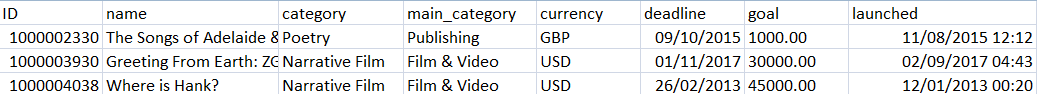
\includegraphics[scale=0.55]{extrait_donnees_partie1.PNG} \end{center}
\begin{center} 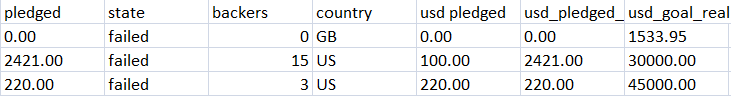
\includegraphics[scale=0.55]{extrait_donnees_partie2.PNG} \end{center}
\noindent Ce jeu de données est intéressant car il a un nombre important d'individus et de variables. De plus, il possède à la fois des variables catégorielles et numériques, ce qui donne de la variété dans les types de variables. \newline

\noindent Pour la suite, nous avons décidé de supprimer les colonnes ID et NAME car ce sont deux variables qui ont des valeurs uniques pour chacun des projets. Nous avons également supprimé les variables GOAL, PLEGED et USD\_PLEGED pour ne garder qu'une unique version de ces variables avec la devise USD.\newline

\noindent Nous conserverons uniquement les projets à l'état "successful" ou "failed" pour l'algorithme adaboost binaire. "Successful" prendra la valeur 1 et "failed" la valeur 0.\newline

\noindent Pour l'extension adaboost.M1 (problèmes multiclasses), nous garderons cette fois-ci tous les individus.


\section{Le protocole expérimental}

Nous souhaitons comparer nos algorithmes implémentés avec d'autres algorithmes de classification supervisé. Ces algorithmes sont issues de la librairie "Scikit-Learn", qui est une librairie de machine learning très prisé des utilisateurs de Python. Les algorithmes choisis vont du plus basique, en partant des moindres carrés ordinaires, et allant vers des algorithmes concurents d'Adaboost.

Les algorithmes testés sont les suivants :
\begin{itemize}
    \item Moindres Carrés ordinaires 
    \item Régression Logistique
    \item Arbre de décision
    \item SVM
    \item Random Forest
    \item Bagging
    \item Ada Boost
\end{itemize}

Tous les algorithmes ont été utilisés sur les mêmes données d'apprentissage et de test, avec le même nombre d'itération. Allant de 1 à 500.

%Pour le protocole expérimental nous avons choisis plusieurs autres algorithmes d'apprentissage supervisé n'utilisant pas le vote par comité. 

%Pour la classification binaire nous avons choisis les algorithmes suivant : 
%Pour la classification multiclasse nous avons choisis les algorithmes suivant : 

%Nous avons entrainé nos 2 algorithmes et les autres algorithmes avec le même nombre d'époques et le même data set. 
%Puis nous avons comparé leurs prédictions avec les prédictions des autres algorithmes choisis à l'aide d'une fonction d'erreur.

%La fonction d'erreur calcule le pourcentage de mauvaises prédictions données sur les données de test. 

\section{Résultats expérimentaux}
Tableau des résultats expérimentaux obtenus avec Adaboost binaire :

\begin{table}[htbp]
    \centering
    \small
    \setlength\tabcolsep{2pt}
    \begin{tabular}{| l | l | l | l | l | l | l |}
    \hline
    Algorithme & 1 itérations & 10 itérations & 50 itérations & 100 itérations & 200 itérations & 500 itérations \\ \hline
    Régression Linéaire & 0.36087 &  0.36087 &  0.36087 & 0.36087 & 0.36087 & 0.36087 \\ \hline
    Régression Logistique & 0.39232 & 0.05242 & 0.00575 & 0.00595 &  0.00595 & 0.00595 \\ \hline
    SVM & 0.27555 & 0.29000 & 0.14666 & 0.07505 & 0.07636 & 0.12707 \\ \hline
    Arbre de décision & 0.00707 & 0.00676 & 0.00656 & 0.00737 & 0.00686 & 0.00707\\ \hline
    Random Forest &  0.04424 & 0.01555 & 0.01171 & 0.01181 & 0.01060 &  0.01131  \\ \hline
    Bagging & 0.00717 & 0.00494 & 0.00414 & 0.00414 & 0.00424 & 0.00424\\ \hline
    Adaboost Scikit-Learn & 0.16202 & 0.06858 &  0.02050 & 0.01383 & 0.00939 & 0.00575\\ \hline
    Adaboost binaire & 0.16202 & 0.08666 & 0.03161 & 0.02131 & 0.01444 & 0.00919\\
    \hline
    \end{tabular}
    \caption{Erreur de prédictions pour des données binaires}
\end{table}

Au vue des résultats de la classification multiclasses on peut se demander pourquoi notre implémentation de l'algorithme M1 ne résulte pas à une diminution de l'erreur au fil des itérations. En effet celui-ci semble converger et ce seulement après quelques itérations. 
Nous avons constater qu'après quelques itérations l'algorithme M1 n'est plus en mesure de produire des classifieurs permettant une estimation supérieur à 0,5. Les classifieurs produits sont ni inférieur à un tirage aléatoire, ni supérieur, mais bien égaux durant toute la suite de l'entrainement. Cela entraine une valeur de beta égale à 1 et cela signifie que ces estimateurs produits ne seront pas interrogés au moment du vote en commité. Voilà pourquoi nous nous retrouvons avec un algorithme qui converge après une ou deux itérations. Au delà de ces itérations l'algorithme ne produit plus d'estimateurs plus performant que l'aléatoire.\\ 

Nous nous sommes interrogés sur ce phénomène et nous avons essayé de mieux le comprendre. Pour cela nous avons créer des jeux de données synthétiques : 
2 produits grâce à la fonction make\_gaussian\_quantile de scikit-learn. La fonction make\_gaussian\_quantile permet de 
générer des échantillons gaussiens isotropes et d'étiqueter les échantillons par quantile. Le premier contenait 10 dimensions et 3 classes, et le second 3 dimensions et 3 classes. Le même phénomène est survenu également sur ces données. \\

Nous avons créer plusieurs datasets de différentes dimensions et de contenant 3 ou plusieurs classes cette fois-ci avec la fonction make\_classification de scikit-learn. la fonction make\_classification génère un problème de classification aléatoire de n-classes. Le code peut être trouvé dans le fichier main\_multiclass.py. Il suffit de d'utiliser la fonction choose\_dataset avec comme argument la fonction générant le dataset souhaité. Les résultats sont meilleurs qu'avec les datasets précédents basés sur des échantillons gaussiens et sont soit proches de l'algorithme adaboost de scikit-learn soit meilleurs parfois. Mais les résultats restent aléatoires et nous n'avons pas deux fois les mêmes résultats lorsque nous lançons l'entrainement. Cela s'explique par le fait que make\_classification introduit une part d'aléatoire dans sa génération de données. \\

Après plusieurs test de datasets créés avec make\_classification nous pensons que l'algorithme M1 a du mal a traité plusieurs classes (supérieur à 3) si de plus celles-ci ne sont pas équilibrées, c'est-à-dire que certaines classes contiennent beaucoup plus d'individus que d'autres.\\ 

Cette observation est en accord avec nos données qui comporte plusieurs classes non équilibrées. \\

Nous avons entrepris de programmer l'algorithme M2 adaboost pour justement constater s'il venait à bout des effet de bords  et des mauvaises performances constatés avec l'algorithme M1. 
Malheureursement nous n'avons pas réussi à aller jusqu'au bout de son implémentation. 
\section{Une discussion scientifique/analyse critique}
Les algorithmes de boosting sont faciles à lire, à implémenter et à interpréter, ce qui rend les interprétations des prédictions facile à manipuler\cite{FreundSchapire1996}. Mais d'un autre coté les algorithmes de boosting soufrent globalement des problèmes d'optimisations et sont fortement influancés par des outliers.\\

Adaboost présente  peu d'inconvénients mais il arrive qu'il soit particulièrement vulnérable au bruit uniforme et aux valeurs aberrantes des données\cite{educba}. 
Un autre inconvénient est que la méthode est presque impossible à mettre à l'échelle. En effet, chaque estimateur fonde sa justesse sur les prédicteurs précédents, ce qui rend la procédure difficile à uniformiser\cite{corporatefinanceinstitute}.\\

Il faut aussi noté les effets liés aux problèmes de déséquilibre de classe\cite{Longadage-2013}. En effet, certains auteurs ont constatés que l'algorithme arrive a faire des séparation même pour des classe mineurs sur des données n'ayant presque pas de frontière mais cependant, la méthode ne peut pas détecter  ce qu'ils ont appeller le "concept à la dérive".\\

Dans notre cas, l'algorithme Adaboost implémenté donne des résultats bien supérieur aux autres algorithmes que sont la Régression lineaire et les SVM. sur les 10 premières itérations, un taux d'erreur de 8\% contre respectivement 29 et 36 pour les SVM et la Régression Linéaire et à 50 itérations, ce taux d'erreur besse de moitié soit à 3\% donc contre 14 et 36\% pour les SVM et la Régression Linéaire.\\
Toute fois sachant que Adaboost combine les propriétés d'optimisations notemment avec les bornes sur les erreurs, les propriétés des SVM car il agit aussi sur les marges entre classe et les propriétés d'algorithmes bayésiens, les résultats que dévrait données notre algorithmes devrait être sans équivoque supérieur voir au coude à coude avec ceux des arbres de décisons. Nous sopposons donc que les résultats sur l'éfficacité d'Adaboost dépendent de la qualité des données mais aussi du type de données. N'ayant pas eu le temps nécessaire de controlé les valeurs aberrantes des données utilisées et nous pouvant affirmé avec mefiance que sur des données saines l'algorithme implementé aurait fait le taux d'erreur le plus bas possibles.

\section{Conclusion}
Dans cette partie nous devons décrire les apports de ce projet (Bonne compréhesion du boosting ?) et les difficultés rencontrées (Trouver un jeu de données ?)

\bibliographystyle{plain}
\bibliography{references}
\end{document}
